\graphicspath{{images/general}}

\section{Diplomarbeit Dokumentation}

\newpage

\section{Eidesstattliche Erklärung}

Ich erkläre an Eides statt, dass ich die vorliegende Diplomarbeit selbständig
und ohne fremde Hilfe verfasst, andere als die angegebenen Quellen und
Hilfsmittel nicht benutzt und die den benutzten Quellen wörtlich und
inhaltlich entnommenen Stellen als solche erkenntlich gemacht habe.

\vspace{1cm}

Rankweil, am 17.05.2025

\begin{figure}[h!]
    \raggedleft
    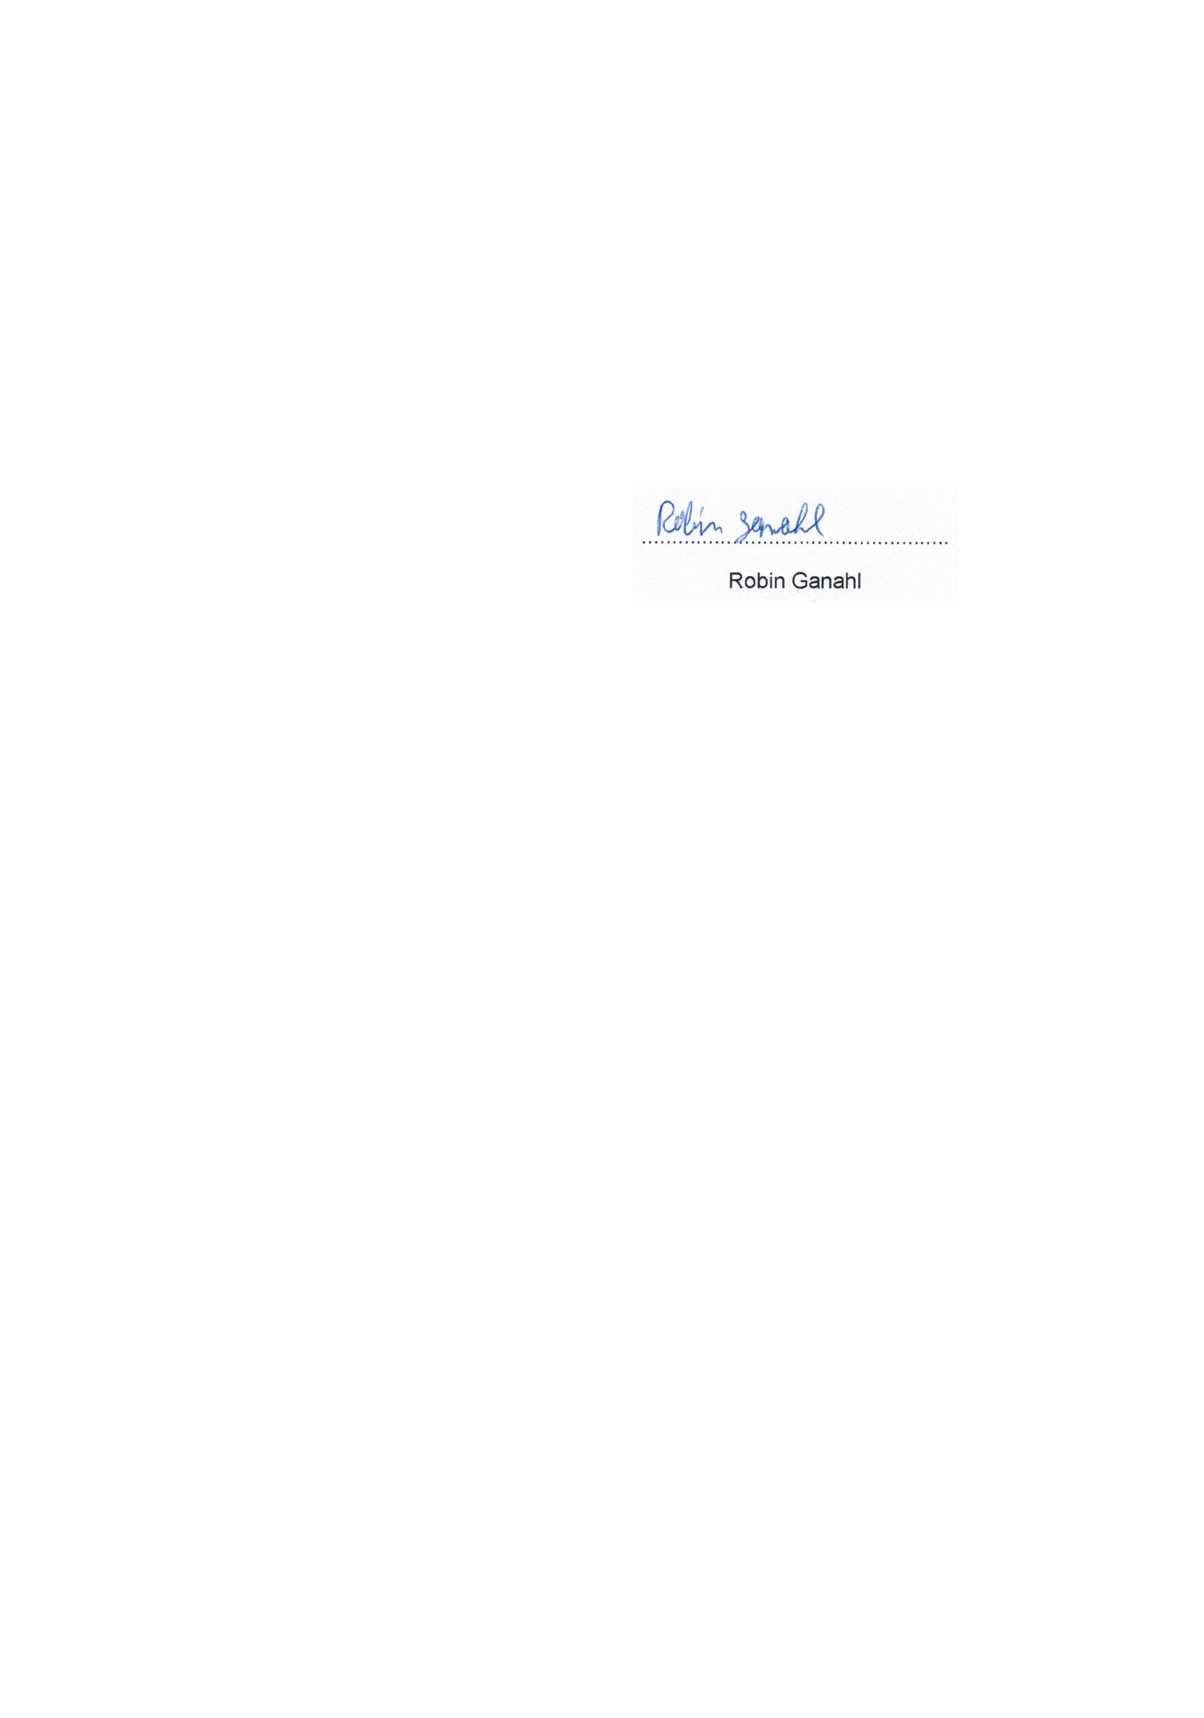
\includegraphics[width=0.3\textwidth]{unterschrift.pdf}
\end{figure}

\newpage

\section{Zusammenfassung}

\subsection{Aufgabenstellung}

Viele Fotobox-Programme sind entweder kostenpflichtig und oft sehr teuer, oder 
als Open-Source-Software verfügbar, aber technisch veraltet und schwer anpassbar.
Diese Einschränkungen machen es schwierig, eine kostengünstige und moderne
Lösung zu finden, die den aktuellen Anforderungen entspricht.
Daher habe ich mich entschieden, im Rahmen meines Maturaprojekts ein eigenes
Fotobox-Programm in C\# zu entwickeln und eine passende Fotobox-Hardware zu bauen.
Mein Ziel ist es, eine benutzerfreundliche, flexible und zeitgemäße Alternative
zu bestehenden Lösungen zu schaffen.

\subsection{Umsetzung}

Für die Umsetzung des Projekts habe ich eine moderne Fotobox-Software in C\# entwickelt,
welche auf einem Windows-PC verwendet werden kann. Die Software unterstützt sowohl Webcams,
beispielsweise die im Laptop integrierte Kamera, als auch professionelle Canon-Spiegelreflexkameras.
Die Fotobox-Hardware besteht aus einer hochwertigen Kamera und einem Laptop mit Touchscreen,
der sowohl zur Bedienung als auch zur Verarbeitung der Bilder dient. 
Für die Benutzerinteraktion wurde eine intuitive Oberfläche mit großen,
leicht verständlichen Buttons entwickelt, um die Bedienung so einfach wie
möglich zu gestalten. Die erstellten Bilder können anschließend direkt
ausgedruckt oder über eine Cloud-Anbindung auf einen Server hochgeladen werden.
Von dort aus können sie bequem auf ein Smartphone heruntergeladen werden.

\subsection{Ergebnisse}

Das Projekt führte zu einer voll funktionsfähigen Fotobox, die eine
benutzerfreundliche und moderne Lösung für Veranstaltungen bietet.
Die Software ermöglicht die Steuerung einer Kamera, das Aufnehmen,
Speichern und Teilen von Fotos sowie den direkten Druck. Dank einer intuitiven
Oberfläche ist die Bedienung einfach und effizient.
Ein besonderer Fokus lag auf der Modularität: Das System kann problemlos
um neue Funktionen, wie Filter oder zusätzliche Hardware erweitert werden.
Zudem wurde eine Cloud-Anbindung integriert, sodass Nutzer ihre Fotos direkt
auf ihr Smartphone herunterladen können. Insgesamt entstand eine kostengünstige,
flexible und zeitgemäße Alternative zu bestehenden Fotobox-Lösungen.